\documentclass[12pt]{article}

% Use packages %
\usepackage{graphicx, courier, amsmath, amssymb, amscd, amsfonts, mathtools, bm, esint, leftidx, extarrows, latexsym, relsize, color, tikz, comment, stmaryrd}
\usepackage[obeyspaces]{url}% http://ctan.org/pkg/url

% Set length %
\setlength{\textwidth}{160mm}
\setlength{\textheight}{235mm}
\setlength{\oddsidemargin}{-0mm}
\setlength{\topmargin}{-10mm}

% Define h-bar %
\newsavebox{\myhbar}
\savebox{\myhbar}{$\hbar$}
\renewcommand*{\hbar}{\mathalpha{\usebox{\myhbar}}}

% Chinese input %
%\usepackage{xeCJK} 
%\setCJKmainfont{微軟正黑體}
%\usepackage[T1]{fontenc}
%\makeatletter

% Equation number %
%\@addtoreset{equation}{section} 
%\renewcommand\theequation{{\thesection}.{\arabic{equation}}}
%\makeatletter 

% Helper Command %
\newcommand{\argmin}{\operatornamewithlimits{argmin}}
\newcommand{\rmnum}[1]{\romannumeral #1} 
\newcommand{\Rmnum}[1]{\expandafter\@slowromancap\romannumeral #1@}
\newcommand{\overbar}[1]{\mkern 1.5mu\overline{\mkern-1.5mu#1\mkern-1.5mu}\mkern 1.5mu}
\makeatother
\newcommand*{\QEDA}{\hfill\ensuremath{\blacksquare}}
\newcommand*{\QEDB}{\hfill\ensuremath{\square}}
\newcommand*{\BmVert}{\bigm\vert}
\newcommand{\bigslant}[2]{{\raisebox{.2em}{$#1$}\left/\raisebox{-.2em}{$#2$}\right.}}
\newcommand{\Nelements}[3]{\left\{ #1, ~ #2, \ldots, ~ #3 \right\}}
\newcommand{\CBrackets}[1]{\left\{#1\right\}}
\newcommand{\SBrackets}[1]{\left[#1\right]}
\newcommand{\ParTh}[1]{\left(#1\right)}
\newcommand{\Ceil}[1]{\left\lceil#1\right\rceil}
\newcommand{\Floor}[1]{\left\lfloor#1\right\rfloor}
\newcommand{\BF}[1]{{\bf#1}}
\newcommand{\Inverse}[1]{{#1}^{-1}}
\newcommand{\Generator}[1]{\left\langle#1\right\rangle}
\newcommand{\AbsVal}[1]{\left|#1\right|}
\newcommand{\VecAbsVal}[1]{\left\|#1\right\|}
\newcommand{\BSlash}[2]{\left.#1\middle\backslash#2\right.}
\newcommand{\Divide}[2]{\left.#1\middle/#2\right.}
\newcommand{\SciNum}[2]{#1\times{10}^{#2}}
\newcommand{\Matrix}[2]{\ParTh{\begin{array}{#1}#2\end{array}}}
\newcommand{\MatrixTwo}[4]{\ParTh{\begin{array}{cc}{#1}&{#2}\\{#3}&{#4}\end{array}}}
\newcommand{\MatrixNByN}[1]{\Matrix{cccc}{{#1}_{11} & {#1}_{12} & \cdots & {#1}_{1n} \\ {#1}_{21} & {#1}_{22} & \cdots & {#1}_{2n} \\ \vdots & \vdots & \ddots & \vdots \\ {#1}_{n1} & {#1}_{n2} & \cdots & {#1}_{nn}}}
\newcommand{\ndiv}{\hspace{-4pt}\not|\hspace{2pt}}
\newcommand{\eqdef}{\xlongequal{\text{def}}}%
\newcount\arrowcount
\newcommand\arrows[1]{\global\arrowcount#1 \ifnum\arrowcount>0
\begin{matrix}\expandafter\nextarrow\fi}
\newcommand\nextarrow[1]{\global\advance\arrowcount-1 \ifx\relax#1\relax\else \xrightarrow{#1}\fi\ifnum\arrowcount=0 \end{matrix}\else\\\expandafter\nextarrow\fi}
\newcommand{\horrule}[1]{\rule{\linewidth}{#1}}

% Tikz settings %
\usetikzlibrary{shapes,arrows}
\tikzstyle{decision} = [diamond, draw, fill=white!20, text width=4.5em, text badly centered, node distance=3cm, inner sep=0pt]
\tikzstyle{block}    = [rectangle, draw, fill=white!20, text width=8em, text centered, rounded corners, minimum height=4em]
\tikzstyle{point}    = [fill = white!20, minimum size=0.5cm]
\tikzstyle{line}     = [draw, -latex']
\tikzstyle{mapsto}   = [draw, |->]
\tikzstyle{cloud}    = [draw, ellipse,fill=red!20, node distance=3cm, minimum height=2em]

\begin{document}

\baselineskip 6.5mm
\setlength{\parindent}{0pt}
\title{ 
\normalfont \normalsize 
\horrule{0.5pt} \\[0.4cm]
\huge { \Huge Machine Learning \\ \large Answer Sheet for Homework 3 }\\ % The assignment title
\horrule{2pt} \\ [0.5cm]
}
\author{ { \Large Da-Min HUANG } \\
{\small R04942045} \\
{\small\textit{Graduate Institute of Communication Engineering, National Taiwan University}}
}
\date{November 16, 2015}
%\allowdisplaybreaks[4]
\maketitle

\subsection*{Problem 1}

Set $\sigma=0.1$ and $d=8$, then we can rewrite the formula to be
\begin{align}
\mathbb{E}_{\mathcal{D}}\SBrackets{E_{\text{in}}\ParTh{\BF{w}_{\text{lin}}}}=0.01\ParTh{1-\dfrac{9}{N}}>0.008\Rightarrow0.2>\dfrac{9}{N}\Rightarrow N>45\Rightarrow N \geq 46
\end{align}

\QEDB

\horrule{0.5pt}

\subsection*{Problem 2}

\begin{enumerate}
	\item[(a)]
	\begin{comment}
	Consider the physical meaning of $\BF{H}$. The projection won't cause the result to be less than zero (one point). So $\BF{H}$ is positive semi-definite.
	\end{comment}
	$\BF{H}$ is positive semi-definite $\Leftrightarrow$ All eigenvalues is non-negative. Refer to choice (c), we have shown the properties.
	\item[(b)]
	Refer to (e), $\BF{H}$ is idempotent matrix. Suppose $\BF{H}^{-1}$ exists, we have
	\begin{align}
	\BF{H}^{-1}\ParTh{\BF{H}^2}=\BF{H}^{-1}\ParTh{\BF{H}}\Rightarrow\BF{H}=\BF{I}
	\end{align}
	Hence, $\BF{H}$ is invertible if and only if $\BF{H}=\BF{I}$. Hence, $\BF{H}$ is not always invertible.
	\begin{comment}
	Consider the physical meaning of $\BF{H}$. The inverse of projection is not injective, which implies that $\BF{H}$ is not always invertible.
	\end{comment}
	\begin{comment}
	Consider $\BF{X}=\Matrix{ccc}{1&2&1\\0&1&1\\1&1&1}$, we have
	\begin{align}
	\BF{H}=\BF{X}\ParTh{\BF{X}^T\BF{X}}^{-1}\BF{X}^T=\Matrix{ccc}{0&0&1\\0&0&1\\1&1&-1}
	\end{align}
	which has no inverse.
	
	Consider the physical meaning of $\BF{H}$. The inverse of projection is not injective, which implies that $\BF{H}$ is not always invertible.
	\end{comment}
	\item[(c)] Refer to choice (e), we have $\BF{H}^2=\BF{H}$. Suppose $\lambda$ is the eigenvalue of some non-zero vector $\vec{v}$,
	\begin{align}
	\BF{H}\vec{v}=\lambda\vec{v}=\BF{H}^2\vec{v}=\BF{H}\ParTh{\lambda\vec{v}}=\lambda\ParTh{\BF{H}\vec{v}}=\lambda^2\vec{v}\Rightarrow\lambda^2=\lambda
	\end{align}
	Hence, the possible results of $\lambda$ is 1 or 0.
	\item[(d)] For a symmetric and idempotent matrix $\BF{H}$, $\text{rank}\ParTh{\BF{H}}=\text{trace}\ParTh{\BF{H}}$, the
	number of non-zero eigenvalues of $\BF{H}$.
	\begin{align}
	\text{trace}\ParTh{\BF{H}}&=\text{trace}\ParTh{\BF{X}\ParTh{\BF{X}^T\BF{X}}^{-1}\BF{X}^T}=\text{trace}\ParTh{\ParTh{\BF{X}^T\BF{X}}^{-1}\BF{X}^T\BF{X}}\\
	&=\text{trace}\ParTh{\BF{I}_{d+1}}=d+1
	\end{align}
	where we have used $\text{trace}\ParTh{\BF{A}\BF{B}}=\text{trace}\ParTh{\BF{B}\BF{A}}$.
	
	Since eigenvalue can only be 0 or 1, so there are $d+1$ eigenvalues of 1.
	\begin{comment}
	Consider the physical meaning of $\BF{H}$. Since there are $d$ features, so at least $d+1$ (since the feature vector contains $x_0$ term) eigenvalues are 1.
	\end{comment}
	\item[(e)] By the definition of $\BF{H}$, we have
	\begin{align}
	\BF{H}^2&=\ParTh{\BF{X}\ParTh{\BF{X}^T\BF{X}}^{-1}\BF{X}^T}\ParTh{\BF{X}\ParTh{\BF{X}^T\BF{X}}^{-1}\BF{X}^T}\\
	&=\BF{X}\ParTh{\BF{X}^T\BF{X}}^{-1}\ParTh{\ParTh{\BF{X}^T\BF{X}}\ParTh{\BF{X}^T\BF{X}}^{-1}}\BF{X}^T\\
	&=\BF{X}\ParTh{\BF{X}^T\BF{X}}^{-1}\BF{X}^T=\BF{H}
	\end{align}
	So
	\begin{align}
	\BF{H}^2=\BF{H}\Rightarrow \BF{H}^{1126}=\BF{H}
	\end{align}
\end{enumerate}

\QEDB

\horrule{0.5pt}

\subsection*{Problem 3}

If $\text{sign}\ParTh{\BF{w}^T\BF{x}}\neq y$, then $y\BF{w}^T\BF{x}<0$ since the sign of $y$ and $\BF{w}^T\BF{x}$ are different. Similarly, if $\text{sign}\ParTh{\BF{w}^T\BF{x}}=y$, then $y\BF{w}^T\BF{x}\geq0$.

\underline{Claim}: $\ParTh{\max\ParTh{0,1-y\BF{w}^T\BF{x}}}^2$ is an upper bound.

\underline{Proof of claim}:

Consider the following cases.
\begin{enumerate}
	\item $\SBrackets{\text{sign}\ParTh{\BF{w}^T\BF{x}}\neq y}=0$
	
	Then $y\BF{w}^T\BF{x}\geq0$. Hence $\ParTh{\max\ParTh{0,1-y\BF{w}^T\BF{x}}}^2\geq0$, which bounds $\SBrackets{\text{sign}\ParTh{\BF{w}^T\BF{x}}\neq y}$.
	\item $\SBrackets{\text{sign}\ParTh{\BF{w}^T\BF{x}}\neq y}=1$
	
	Then $y\BF{w}^T\BF{x}<0$. Hence $\ParTh{\max\ParTh{0,1-y\BF{w}^T\BF{x}}}^2=\ParTh{1-y\BF{w}^T\BF{x}}^2>1$, which bounds $\SBrackets{\text{sign}\ParTh{\BF{w}^T\BF{x}}\neq y}$.
\end{enumerate}

\QEDB

\horrule{0.5pt}

\subsection*{Problem 4}

Set $y\BF{w}^T\BF{x}\coloneqq z$. Consider $\max\ParTh{0,-y\BF{w}^T\BF{x}}=\max\ParTh{0,-z}\coloneqq f\ParTh{z}$. We have $f\ParTh{z}=-z$ if $z\leq0$, else $f\ParTh{z}=0$. So 
\begin{align}
\lim\limits_{z\rightarrow0^{-}}\dfrac{f\ParTh{z}-f\ParTh{0}}{z-0}=\dfrac{-z-0}{z-0}=-1,~\lim\limits_{z\rightarrow0^{+}}\dfrac{f\ParTh{z}-f\ParTh{0}}{z-0}=\dfrac{0-0}{z-0}=0
\end{align}
Hence, $f\ParTh{z}$ is not differentiable at $z=0$.

\QEDB

\horrule{0.5pt}

\subsection*{Problem 5}

\underline{Calim}: $\max\ParTh{0, -y\BF{w}^T\BF{x}}$ results in PLA.

\underline{Proof of claim}:

Consider following cases.
\begin{enumerate}
	\item $y = \text{sign}\ParTh{\BF{w}^T\BF{x}}$. PLA update term is 0.
	
	Then we have $y\BF{w}^T\BF{x} > 0$. So
	\begin{align}
	\max\ParTh{0, -y\BF{w}^T\BF{x}}=0
	\end{align}
	\item $y \neq \text{sign}\ParTh{\BF{w}^T\BF{x}}$. PLA update term is $y\BF{x}$.
	
	Then we have $y\BF{w}^T\BF{x} < 0$. So
	\begin{align}
	\max\ParTh{0, -y\BF{w}^T\BF{x}}=-y\BF{w}^T\BF{x}\Rightarrow-\nabla_{\BF{w}}\max\ParTh{0, -y\BF{w}^T\BF{x}}=y\BF{x}
	\end{align}
\end{enumerate}
\begin{comment}
Set $\eta=1$ and let $\BF{w}^T_t\BF{x}_n$ be large enough, we have
\begin{align}
\lim\limits_{\BF{w}^T_t\BF{x}_n\rightarrow\infty}\theta\ParTh{-y_n\BF{w}^T_t\BF{x}_n}&=\lim\limits_{\BF{w}^T_t\BF{x}_n\rightarrow\infty}\dfrac{1}{1+\exp\ParTh{y_n\BF{w}^T_t\BF{x}_n}}=\left\{\begin{array}{ll}
1,&\text{if sign}\ParTh{\BF{w}^T_t\BF{x}_n}\neq y_n\\
0,&\text{if sign}\ParTh{\BF{w}^T_t\BF{x}_n}= y_n
\end{array}\right.\\
&=\left\llbracket{y_n\neq\text{sign}\ParTh{\BF{w}^T_t\BF{x}_n}}\right\rrbracket
\end{align}
\end{comment}

\QEDB

\horrule{0.5pt}

\subsection*{Problem 6}

\begin{align}
\nabla E(0,0) &= \left.\ParTh{\frac{\partial E}{\partial u},\frac{\partial E}{\partial v}}\right|_{\ParTh{0,0}}\\
&= \left.\ParTh{e^{u}+ve^{uv}+2u-2v-3,2e^{2v}+ue^{uv}-2u+4v-2}\right|_{\ParTh{0,0}}\\
&=\ParTh{-2,0}
\end{align}

\QEDB

\horrule{0.5pt}

\subsection*{Problem 7}

I write a program Q07.py to calculate the result by using
\begin{align}
\ParTh{u_{t+1},v_{t+1}}=\ParTh{u_t,v_t}-0.01\nabla E\ParTh{u_t,v_t}
\end{align}
iteratively.
\begin{align}
\ParTh{u_1,v_1}&=\ParTh{0,0}-0.01\nabla E\ParTh{0,0}=\ParTh{0.02,0}\\
\ParTh{u_2,v_2}&=\ParTh{0.02,0}-0.01\nabla E\ParTh{0.02,0}\approx\ParTh{0.039398,0.0002}\\
\ParTh{u_3,v_3}&\approx\ParTh{0.039398,0.0002}-0.01\nabla E\ParTh{0.039398,0.0002}\\&\approx\ParTh{0.0582102,0.000577975}\\
\ParTh{u_4,v_4}&\approx\ParTh{0.0764524,0.00111381}\\
\ParTh{u_5,v_5}&\approx\ParTh{0.09414,0.00178911}\\
E\ParTh{u_5,v_5}&\approx2.825
\end{align}

\QEDB

\horrule{0.5pt}

\subsection*{Problem 8}

\begin{align}
\nabla E(0,0) &= \ParTh{\frac{\partial E}{\partial u},\frac{\partial E}{\partial v}}\\
&=\ParTh{e^{u}+ve^{uv}+2u-2v-3,2e^{2v}+ue^{uv}-2u+4v-2}
\end{align}
From this we compute the Hessian matrix
\begin{align}
\nabla^2E\ParTh{u,v}=\Matrix{cc}{e^{u}+v^2e^{uv}+2&\ParTh{uv+1}e^{uv}-2\\\ParTh{uv+1}e^{uv}-2&4e^{2v}+u^2e^{uv}+4}
\end{align}
So
\begin{align}
\hat{E}\ParTh{\Delta u,\Delta v}&=E\ParTh{0,0}+\nabla E\ParTh{0,0}\cdot\ParTh{\Delta u,\Delta v}+\dfrac{1}{2}\ParTh{\Delta u,\Delta v}\nabla^2E\ParTh{0,0}\Matrix{c}{\Delta u\\\Delta v}\\
&=3-2\Delta u+\dfrac{1}{2}\ParTh{\Delta u,\Delta v}\Matrix{cc}{3&-1\\-1&8}\Matrix{c}{\Delta u\\\Delta v}\\
&=\dfrac{3}{2}\ParTh{\Delta u}^2+4\ParTh{\Delta v}^2-\Delta u\Delta v-2\Delta u+0\Delta v+3
\end{align}

\QEDB

\horrule{0.5pt}

\subsection*{Problem 9}

\underline{Claim}: $-\ParTh{\nabla^2E\ParTh{u,v}}^{-1}\nabla E\ParTh{u,v}$ is the Newton direction.

\underline{Proof of claim}:
\begin{align}
\dfrac{\partial\hat{E}\ParTh{\Delta u,\Delta v}}{\partial\ParTh{\Delta u,\Delta v}}&=\nabla E\ParTh{u,v}+\nabla^2E\ParTh{u,v}\ParTh{\Delta u,\Delta v}=0\\
\Rightarrow\ParTh{\Delta u,\Delta v}&=-\ParTh{\nabla^2E\ParTh{u,v}}^{-1}\nabla E\ParTh{u,v}
\end{align}
\begin{comment}
Now we have
\begin{align}
\hat{E}\ParTh{\Delta u,\Delta v}&=\dfrac{3}{2}\ParTh{\Delta u}^2+4\ParTh{\Delta v}^2-\Delta u\Delta v-2\Delta u+3
\end{align}
So
\begin{align}
\left.\begin{array}{l}
\dfrac{\partial\hat{E}}{\partial\ParTh{\Delta u}}=3\Delta u-\Delta v-2=0\\
\dfrac{\partial\hat{E}}{\partial\ParTh{\Delta v}}=8\Delta v-\Delta u=0\\
\end{array}\right\}\Rightarrow\Delta u=\dfrac{16}{23},~\Delta v=\dfrac{2}{23}
\end{align}
\end{comment}

\QEDB

\horrule{0.5pt}

\subsection*{Problem 10}

I write a program Q10.py to calculate the result by using
\begin{align}
\ParTh{u_{t+1},v_{t+1}}=\ParTh{u_t,v_t}-\ParTh{\nabla^2E\ParTh{u_t,v_t}}^{-1}\nabla E\ParTh{u_t,v_t}
\end{align}
iteratively.
\begin{align}
\ParTh{u_1,v_1}&\approx\ParTh{0.695652173913, 0.0869565217391}\\
\ParTh{u_2,v_2}&\approx\ParTh{0.613762221112, 0.0711078990173}\\
\ParTh{u_3,v_3}&\approx\ParTh{0.611812859879, 0.0705000613365}\\
\ParTh{u_4,v_4}&\approx\ParTh{0.611811717261, 0.0704995471019}\\
\ParTh{u_5,v_5}&\approx\ParTh{0.61181171726, 0.0704995471016}\\
E\ParTh{u_5,v_5}&\approx2.36082334564
\end{align}
This equals to the value of Problem 7 after 746 updates.

\QEDB

\horrule{0.5pt}

\subsection*{Problem 11}

Write a program Q11.py to test, $\CBrackets{\BF{x}_1,\BF{x}_2,\BF{x}_3,\BF{x}_4,\BF{x}_5,\BF{x}_6}$ is the biggest subset that can be shattered by the union of quadratic, linear, or constant hypotheses of $\BF{x}$ by feature form of
\begin{align}
\Phi\ParTh{\BF{x}}=\ParTh{1,x_1,x_2,x^2_1,x_1x_2,x^2_2}
\end{align}
Then I ran the PLA and all cases are stasified. The $\BF{w}$ for $2^6=64$ cases are
\begin{align}
\begin{array}{llll}
\left[ 0,  0,  0,  0,  0,  0\right],~&\left[ 0,  1,  0,  1,  0, -4\right],~&\left[ 1,  0,  1, -2, -1, -1\right],~&\left[ 2,  0,  0,  0,  0, -2\right],\\
\left[-1, -2,  0,  0, -2,  0\right],~&\left[ 0,  0,  1,  2, -1, -3\right],~&\left[ 1, -1,  2, -1, -2,  0\right],~&\left[ 2, -1,  1,  1, -1, -3\right],\\
\left[ 0,  0, -2,  0,  2,  0\right],~&\left[ 0,  0, -3,  2,  3, -3\right],~&\left[ 1, -1, -2, -1,  2,  0\right],~&\left[ 2,  0, -2,  0,  2, -2\right],\\
\left[-1, -4,  0,  0,  0,  0\right],~&\left[ 0, -2, -1,  4,  1, -3\right],~&\left[ 1, -2, -1,  0,  1,  1\right],~&\left[ 3, -2,  0,  2,  0, -4\right],\\
\left[-1,  1,  0, -1, -2,  0\right],~&\left[ 0,  2,  0,  0, -2,  0\right],~&\left[ 1,  1, -2, -3, -2,  0\right],~&\left[ 1,  1, -1, -1, -3, -1\right],\\
\left[-1,  0,  1,  0, -3,  1\right],~&\left[ 0,  1,  0,  1, -4,  0\right],~&\left[ 1, -1,  1, -1, -3,  1\right],~&\left[ 1,  0,  0,  0, -4,  0\right],\\
\left[ 0,  0, -3,  0,  1,  1\right],~&\left[ 0,  1, -4,  1,  0,  0\right],~&\left[ 1, -1, -3, -1,  1,  1\right],~&\left[ 1,  0, -4,  0,  0,  0\right],\\
\left[ 0, -1, -2,  1,  0,  2\right],~&\left[ 0,  0, -3,  2, -1,  1\right],~&\left[ 1, -1, -1, -1, -1,  1\right],~&\left[ 1, -1, -3,  1, -1,  1\right],\\
\left[ 0,  0,  2,  0,  2,  0\right],~&\left[ 0,  2,  3,  0,  1, -1\right],~&\left[ 1,  0,  3, -2,  1, -1\right],~&\left[ 1,  1,  3, -1,  1, -1\right],\\
\left[-1,  0,  4,  0,  0,  0\right],~&\left[ 0,  1,  4,  1,  0,  0\right],~&\left[ 1, -1,  4, -1,  0,  0\right],~&\left[ 1,  0,  4,  0,  0,  0\right],\\
\left[ 0,  0,  0,  0,  4,  0\right],~&\left[ 0,  1,  0,  1,  4,  0\right],~&\left[ 1, -1,  0, -1,  4,  0\right],~&\left[ 1,  0,  0,  0,  4,  0\right],\\
\left[ 0, -1,  1,  1,  3,  1\right],~&\left[ 0,  0,  1,  2,  3,  1\right],~&\left[ 1, -2,  1,  0,  3,  1\right],~&\left[ 1, -1,  1,  1,  3,  1\right],\\
\left[-2,  2,  0, -2,  0,  4\right],~&\left[ 0,  4,  0,  0,  0,  0\right],~&\left[ 1,  2,  1, -4, -1,  3\right],~&\left[ 2,  4,  0,  0,  0,  0\right],\\
\left[-1,  0,  2,  0, -2,  2\right],~&\left[ 0,  1,  3,  1, -1,  1\right],~&\left[ 1,  0,  3, -2, -3,  3\right],~&\left[ 1,  1,  3,  1, -1,  1\right],\\
\left[-1,  1, -1, -1,  1,  3\right],~&\left[ 0,  3, -1,  1,  1,  1\right],~&\left[ 1,  0, -1, -2,  1,  3\right],~&\left[ 1,  2,  0,  0,  2,  0\right],\\
\left[-1,  0,  0,  0,  0,  2\right],~&\left[ 0,  1,  1,  1,  1,  1\right],~&\left[ 1, -1,  0, -1,  0,  4\right],~&\left[ 1,  1,  1,  1,  1,  1\right]
\end{array}
\end{align}
\begin{comment}
If $\BF{x}_1$ and $\BF{x}_3$ are on the same side, then $\BF{x}_2$ and $\BF{x}_4$ can't be the same side. So $\CBrackets{\BF{x}_1,\BF{x}_2,\BF{x}_3}$ is the biggest subset that can be shattered by the union of quadratic, linear, or constant hypotheses of $\BF{x}$.
\begin{align}
\BF{x}_4&=-\BF{x}_2\\
\BF{x}_5&=\BF{x}_1+\BF{x}_3\\
\BF{x}_6&=\dfrac{1}{2}\ParTh{\BF{x}_1+\BF{x}_2}
\end{align}
So $\CBrackets{\BF{x}_1,\BF{x}_2,\BF{x}_3}$ is the biggest subset that can be shattered by the union of quadratic, linear, or constant hypotheses of $\BF{x}$.
\end{comment}

\QEDB

\horrule{0.5pt}

\subsection*{Problem 12}

By the transform, we have $\ParTh{\Phi\ParTh{\BF{x}}}_i=z_i=\ParTh{0,\ldots,\underbrace{1}_{i\text{-th term}},\ldots,0}$. To shatter the original $N$ points, we can assign $w_i$ to be positive or negative to get $\BF{x}_i$ $\circ$ or $\times$.

So, this transform shatter any $N$ points. Hence $d_{vc}\ParTh{\mathcal{H}_\Phi}=\infty$.

\QEDB

\horrule{0.5pt}

\subsection*{Problem 13}

The average $E_{\text{in}}$ is 0.503979.
\begin{figure}[h]
	\centering
	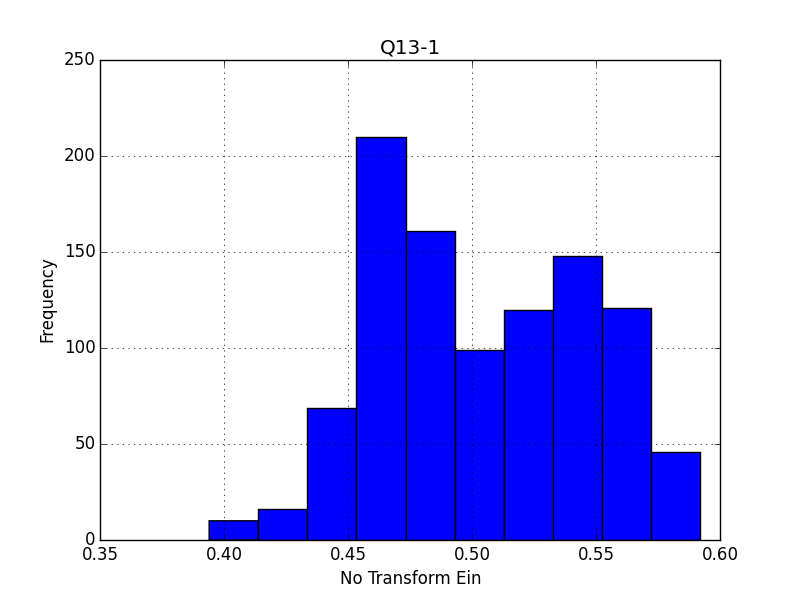
\includegraphics[scale=0.3]{Q13-1.png}
	\caption{Q13 histogram}
	\label{Q13}
\end{figure}

After feature transform, we have
\begin{align}
\tilde{\BF{w}}=&\left[-0.991720295,\SciNum{-3.00273423}{-4},\SciNum{-1.31851902}{-3},\right.\\
\nonumber
&~\left.\SciNum{1.09524038}{-3},1.55703088,1.55594342\right]
\end{align}
with new average $E_{\text{in}}=0.124126$.

\QEDB

\horrule{0.5pt}

\subsection*{Problem 14}

The average $\tilde{\BF{w}}_{3}={0.06306984}$.
\begin{figure}[h]
	\centering
	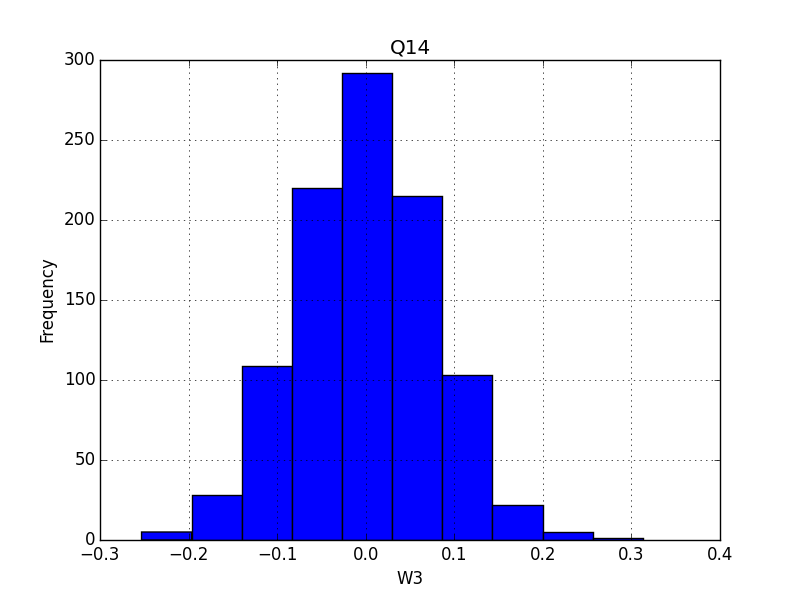
\includegraphics[scale=0.3]{Q14.png}
	\caption{Q14 histogram}
	\label{Q14}
\end{figure}

\QEDB

\horrule{0.5pt}

\newpage
\subsection*{Problem 15}

The average $E_{\text{out}}=0.126195$.
\begin{figure}[h]
	\centering
	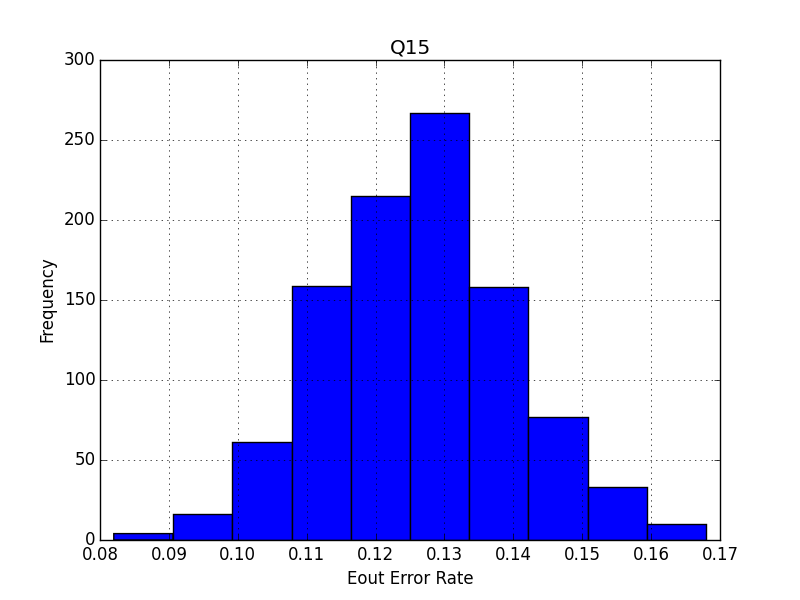
\includegraphics[scale=0.3]{Q15.png}
	\caption{Q15 histogram}
	\label{Q15}
\end{figure}

\QEDB

\horrule{0.5pt}

\subsection*{Problem 16}

Sum the minimized negative log likelihood $h_y$, which is $\min_y\ParTh{-\ln\ParTh{h_y}}$, we have
\begin{align}
E_{\text{in}}&=\dfrac{1}{N}\sum_{n=1}^{N}\ParTh{-\ln\ParTh{\dfrac{\exp\ParTh{\BF{w}^T_{y_n}\BF{x}_n}}{\sum_{i=1}^{K}\exp\ParTh{\BF{w}^T_i\BF{x}_n}}}}\\
&=\dfrac{1}{N}\sum_{n=1}^{N}\ParTh{\ln\ParTh{\sum_{i=1}^{K}\exp\ParTh{\BF{w}^T_i\BF{x}_n}}-\BF{w}^T_{y_n}\BF{x}_n}
\end{align}

\QEDB

\horrule{0.5pt}

\subsection*{Problem 17}

\begin{align}
\dfrac{\partial E_{\text{in}}}{\partial \BF{w}_i}&=\dfrac{1}{N}\sum_{n=1}^{N}\dfrac{\partial}{\partial \BF{w}_i}\ParTh{\ln\ParTh{\sum_{i=1}^{K}\exp\ParTh{\BF{w}^T_i\BF{x}_n}}-\BF{w}^T_{y_n}\BF{x}_n}\\
&=\dfrac{1}{N}\sum_{n=1}^{N}\ParTh{\dfrac{1}{\sum_{i=1}^{K}\exp\ParTh{\BF{w}^T_i\BF{x}_n}}\dfrac{\partial}{\partial \BF{w}_i}\exp\ParTh{\BF{w}^T_i\BF{x}_n}-\dfrac{\partial}{\partial \BF{w}_i}\BF{w}^T_{y_n}\BF{x}_n}\\
&=\dfrac{1}{N}\sum_{n=1}^{N}\ParTh{\dfrac{\exp\ParTh{\BF{w}^T_i\BF{x}_n}}{\sum_{i=1}^{K}\exp\ParTh{\BF{w}^T_i\BF{x}_n}}\BF{x}_n-\left\llbracket y_n=i\right\rrbracket\BF{x}_n}\\
&=\dfrac{1}{N}\sum_{n=1}^{N}\ParTh{h_i\ParTh{\BF{x}_n}-\left\llbracket y_n=i\right\rrbracket}\BF{x}_n
\end{align}

\QEDB

\horrule{0.5pt}

\subsection*{Problem 18}

The $E_{\text{out}}=0.475$ with
\begin{align}
\tilde{\BF{w}}=&\left[0.01878417, -0.01260595,  0.04084862, -0.03266317,  0.01502334,\right.\\
\nonumber
&~-0.03667437,0.01255934,  0.04815065, -0.02206419,  0.02479605,\\
\nonumber
&~0.06899284,  0.0193719,
-0.01988549, -0.0087049,   0.04605863,\\
\nonumber
&~\left.0.05793382,  0.061218,   -0.04720391,
0.06070375, -0.01610907, -0.03484607\right]
\end{align}

\QEDB

\horrule{0.5pt}

\subsection*{Problem 19}

The $E_{\text{out}}=0.220$ with
\begin{align}
\tilde{\BF{w}}=&\left[-0.00385379, -0.18914564,  0.26625908, -0.35356593,  0.04088776,\right.\\
\nonumber
&~-0.3794296,
0.01982783,  0.33391527, -0.26386754,  0.13489328,\\
\nonumber
&~0.4914191,   0.08726107,
-0.25537728, -0.16291797,  0.30073678,\\
\nonumber
&~\left.0.40014954,  0.43218808, -0.46227968,
0.43230193, -0.20786372, -0.36936337\right]
\end{align}

\QEDB

\horrule{0.5pt}

\subsection*{Problem 20}

The $E_{\text{out}}=0.473$ with
\begin{align}
\tilde{\BF{w}}=&\left[0.01826899, -0.01308051,  0.04072894, -0.03295698,  0.01498363,\right.\\
\nonumber
&~-0.03691042,0.01232819,  0.04791334, -0.02244958,  0.02470544,\\
\nonumber
&~0.06878235,  0.01897378,-0.02032107, -0.00901469,  0.04589259,\\
\nonumber
&~\left.0.05776824,  0.06102487, -0.04756147,0.06035018, -0.01660574, -0.03509342\right]
\end{align}

\QEDB

\horrule{0.5pt}

\subsection*{Problem 21}

\begin{align}
\BF{h}^T\BF{y}=\sum_{i=1}^{N}h\ParTh{\BF{x}_i}y_i
\end{align}
We just need two times queries to obtain $\BF{h}^T\BF{y}$.

First, take some $h^\prime$ such that $h^\prime\ParTh{\BF{x}_i}=0$, $\forall i$. Then we have
\begin{align}
\text{RMSE}\ParTh{h^\prime}=\sqrt{\dfrac{1}{N}\sum_{i=1}^{N}\ParTh{y_i-h^\prime\ParTh{\BF{x_i}}}^2}=\sqrt{\dfrac{1}{N}\sum_{i=1}^{N}y^2_i}\Rightarrow\sum_{i=1}^{N}y^2_i=N\ParTh{\text{RMSE}\ParTh{h^\prime}}^2
\end{align}
Second, query for some $h$,
\begin{align}
\text{RMSE}\ParTh{h}&=\sqrt{\dfrac{1}{N}\sum_{i=1}^{N}\ParTh{y_i-h\ParTh{\BF{x_i}}}^2}\\
N\ParTh{\text{RMSE}\ParTh{h}}^2&=\sum_{i=1}^{N}\ParTh{y_i-h\ParTh{\BF{x_i}}}^2=\sum_{i=1}^{N}y^2_i-2h\ParTh{\BF{x}_i}y_i+h^2\ParTh{\BF{x_i}}\\
\Rightarrow\BF{h}^T\BF{y}&=-\dfrac{1}{2}\ParTh{N\ParTh{\text{RMSE}\ParTh{h}-\text{RMSE}\ParTh{h^\prime}}^2-\sum_{i=1}^{N}h^2\ParTh{\BF{x_i}}}
\end{align}
where we have known the value of $\sum_{i=1}^{N}h^2\ParTh{\BF{x_i}}$ since we have already known all $\BF{x}_i$.

\QEDB

\horrule{0.5pt}

\subsection*{Problem 22}

To find $\min_{\BF{w}}\text{RMSE}\ParTh{H}$, we need to find $\nabla\text{RMSE}\ParTh{H}=0$.
\begin{align}
\nabla\text{RMSE}\ParTh{H}=0&\Rightarrow\dfrac{\partial}{\partial w_k}\sum_{i=1}^{N}\ParTh{y_i-\sum_{k=1}^{K}w_kh_k\ParTh{\BF{x_i}}}^2=0, \forall k\\
&\Rightarrow2\sum_{i=1}^{N}\ParTh{h_k\ParTh{\BF{x}_i}y_i-h_k\ParTh{\BF{x}_i}\sum_{k=1}^{K}w_kh_k\ParTh{\BF{x_i}}}=0, \forall k
\end{align}
Hence, we need to know the value of $\BF{h}^T_k\BF{y}$ for all $k$. Hence, follow the conclusion above, we need to query for $K+1$ times, where the $+1$ is for querying the value of $\sum_{i=1}^{N}y^2_i$. The derivation steps are
\begin{enumerate}
	\item First, use some hypothesis $h^\prime$ such that $h^\prime\ParTh{\BF{x}_i}=0$, $\forall i$ to get the value of $\sum_{i=1}^{N}y^2_i$.
	\item Second, query for $\text{RMSE}\ParTh{h_k}$, $\forall k$, costs $K$ times query. Then we have all $\BF{h}^T_k\BF{y}$.
\end{enumerate}
Hence, we have
\begin{align}
\BF{h}^T_k\BF{y}-\sum_{i=1}^{N}\ParTh{h_k\ParTh{\BF{x}_i}\sum_{k=1}^{K}w_kh_k\ParTh{\BF{x}_i}}=0,~\forall k
\end{align}
Then we can solve the value of $\BF{w}$ to get the minimized value.
\begin{comment}
\begin{align}
\text{RMSE}\ParTh{H}=\sqrt{\dfrac{1}{N}\sum_{i=1}^{N}\ParTh{y_i-\sum_{k=1}^{K}w_kh_k\ParTh{\BF{x_i}}}}
\end{align}
\end{comment}

\QEDB

\horrule{0.5pt}

\section*{Reference}

\begin{enumerate}

\item[{[1]}] Lecture Notes by Hsuan-Tien LIN, Department of Computer Science and Information Engineering, National Taiwan University, Taipei 106, Taiwan.

%\item[{[2]}] Three proofs of Sauer-Shelah Lemma. (n. d. ). Retrieved Fall, 2010, from \url{http://www.cse.buffalo.edu/~hungngo/classes/2010/711/lectures/sauer.pdf}

\end{enumerate}

\end{document}